\chapter{Related Technologies and Theoretical Foundations}
\label{cha:related_technologies}

This chapter provides a comprehensive review of the fundamental technologies and theoretical foundations underlying the proposed hybrid Transformer-LSTM model. The chapter is organized into two main sections that examine the core architectures essential to this research. First, we explore Long Short-Term Memory (LSTM) networks, discussing their gating mechanisms, bidirectional capabilities, and their effectiveness in capturing sequential dependencies in time-series data. Second, we examine the Transformer architecture, focusing on its self-attention mechanism, multi-head attention, and encoder structure that enables parallel processing and global context modeling. Together, these technologies form the theoretical foundation for understanding how their complementary strengths can be combined to create a more robust fault diagnosis system.

\section{Long Short-Term Memory Networks (LSTM)}
\label{sec:related_technologies:lstm}

This section reviews recurrent neural networks (RNNs) and the challenges of training them, introduces the Long Short-Term Memory (LSTM) architecture and its gating mechanism, discusses the strengths and limitations of LSTMs for time-series modeling, and explains the principle of Bidirectional LSTM (Bi-LSTM).

\subsection{RNN Basics and the Vanishing/Exploding\\ Gradient Problem}
An RNN processes a sequence \(\mathbf{x}_t\) by maintaining a hidden state \(\mathbf{h}_t\) that is updated recurrently as:
\begin{equation}
\mathbf{h}_t = \phi(\mathbf{W}_{xh}\,\mathbf{x}_t + \mathbf{W}_{hh}\,\mathbf{h}_{t-1} + \mathbf{b}_h)
\label{eq:rnn_update}
\end{equation}
where \(\phi\) is a nonlinearity. Training is typically done via backpropagation through time (BPTT), which unrolls the network over temporal steps. In long sequences, repeated multiplication by Jacobians leads to gradients that either shrink towards zero (vanish) or grow uncontrollably (explode), hampering the learning of long-range dependencies and causing optimization instability \cite{pascanu2013difficulty}. Gradient clipping mitigates exploding gradients, but vanishing gradients remain a central obstacle for standard RNNs to capture dependencies spanning many time steps.

More concretely, the gradient across \(k\) steps contains products like:
\begin{equation}
\prod_{i=1}^{k} \frac{\partial \mathbf{h}_{t-i+1}}{\partial \mathbf{h}_{t-i}}
\label{eq:gradient_product}
\end{equation}
When the spectral radius of the recurrent Jacobian is smaller (greater) than one on average, gradients decay (blow up) exponentially with \(k\), which explains why plain RNNs struggle with long-term credit assignment. Practical workarounds include truncated BPTT (limiting the backpropagated horizon), gradient clipping for stability, careful initialization (e.g., orthogonal \(\mathbf{W}_{hh}\)), and using gates or skip/residual connections to create more favorable gradient pathways \cite{pascanu2013difficulty}. These heuristics help but do not fully resolve vanishing gradients in vanilla RNNs, which motivates gated architectures such as the LSTM.

From a training perspective, backpropagation through time over a window of length \(K\) costs roughly:
\begin{equation}
\mathcal{O}(K \cdot (d_x d_h + d_h^2))
\label{eq:bptt_complexity}
\end{equation}
per sequence, where \(d_x\) and \(d_h\) are the input and hidden dimensions. Truncated BPTT chooses a moderate \(K\) (e.g., 50--200 steps) to balance long-range learning with computational and memory budgets. Gradient clipping commonly constrains the global norm:
\begin{equation}
\lVert \nabla \rVert_2 \leftarrow \min(\lVert \nabla \rVert_2, \tau)
\label{eq:gradient_clipping}
\end{equation}
to avoid instability when occasional large Jacobian products arise.

Finally, activation choices matter: saturating nonlinearities (sigmoid, tanh) have derivatives bounded by \((0, 0.25]\) and \((0, 1]\) respectively, which can compound vanishing; non-saturating alternatives (ReLU) improve gradient flow but complicate recurrent stability and may cause unbounded activations without care. These trade-offs further motivate gated RNNs that provide an explicit additive path for gradients.

\subsection{LSTM Gates and Working Mechanism}

LSTM networks address vanishing gradients by introducing an additive memory pathway---the cell state \(\mathbf{c}_t\)---and multiplicative gates that regulate information flow \cite{hochreiter1997long}. 

\paragraph{Core LSTM Equations.} At each time step, the LSTM computes the following gates and states:
\begin{align}
\mathbf{f}_t &= \sigma(\mathbf{W}_f [\mathbf{x}_t, \mathbf{h}_{t-1}] + \mathbf{b}_f) &&\text{(forget gate)}\\
\mathbf{i}_t &= \sigma(\mathbf{W}_i [\mathbf{x}_t, \mathbf{h}_{t-1}] + \mathbf{b}_i) &&\text{(input gate)}\\
\tilde{\mathbf{c}}_t &= \tanh(\mathbf{W}_c [\mathbf{x}_t, \mathbf{h}_{t-1}] + \mathbf{b}_c) &&\text{(candidate state)}\\
\mathbf{c}_t &= \mathbf{f}_t \odot \mathbf{c}_{t-1} + \mathbf{i}_t \odot \tilde{\mathbf{c}}_t &&\text{(cell update)}\\
\mathbf{o}_t &= \sigma(\mathbf{W}_o [\mathbf{x}_t, \mathbf{h}_{t-1}] + \mathbf{b}_o) &&\text{(output gate)}\\
\mathbf{h}_t &= \mathbf{o}_t \odot \tanh(\mathbf{c}_t) &&\text{(hidden state)}
\end{align}

where \(\sigma\) denotes the logistic sigmoid function and \(\odot\) represents element-wise multiplication.

\paragraph{Key Innovation: Additive Cell State.} The critical innovation lies in the cell-state update equation \(\mathbf{c}_t = \mathbf{f}_t \odot \mathbf{c}_{t-1} + \mathbf{i}_t \odot \tilde{\mathbf{c}}_t\), which preserves information through additive interactions modulated by gates. This creates a constant error carousel that supports more stable gradient flow across time. Unlike vanilla RNNs that suffer from repeated matrix multiplications during backpropagation, this additive update mechanism provides an almost unattenuated pathway for gradients, enabling LSTMs to learn both short- and moderately long-range temporal dependencies \cite{hochreiter1997long}.

\paragraph{Gate Functions and Information Flow.} As illustrated in Figure~\ref{fig:lstm_cell_diagram}, each gate serves a specific purpose:
\begin{itemize}
    \item \textbf{Forget gate} \(\mathbf{f}_t\): Controls what information to discard from the cell state
    \item \textbf{Input gate} \(\mathbf{i}_t\): Determines which values to update in the cell state
    \item \textbf{Candidate state} \(\tilde{\mathbf{c}}_t\): Generates new candidate values to be added
    \item \textbf{Output gate} \(\mathbf{o}_t\): Controls which parts of the cell state to output
\end{itemize}

The gates jointly regulate how information is retained, written, and exposed from the cell state, providing a practical implementation of the mathematical formulations above.

% External figure referenced above
\begin{figure}[tbp]
\centering
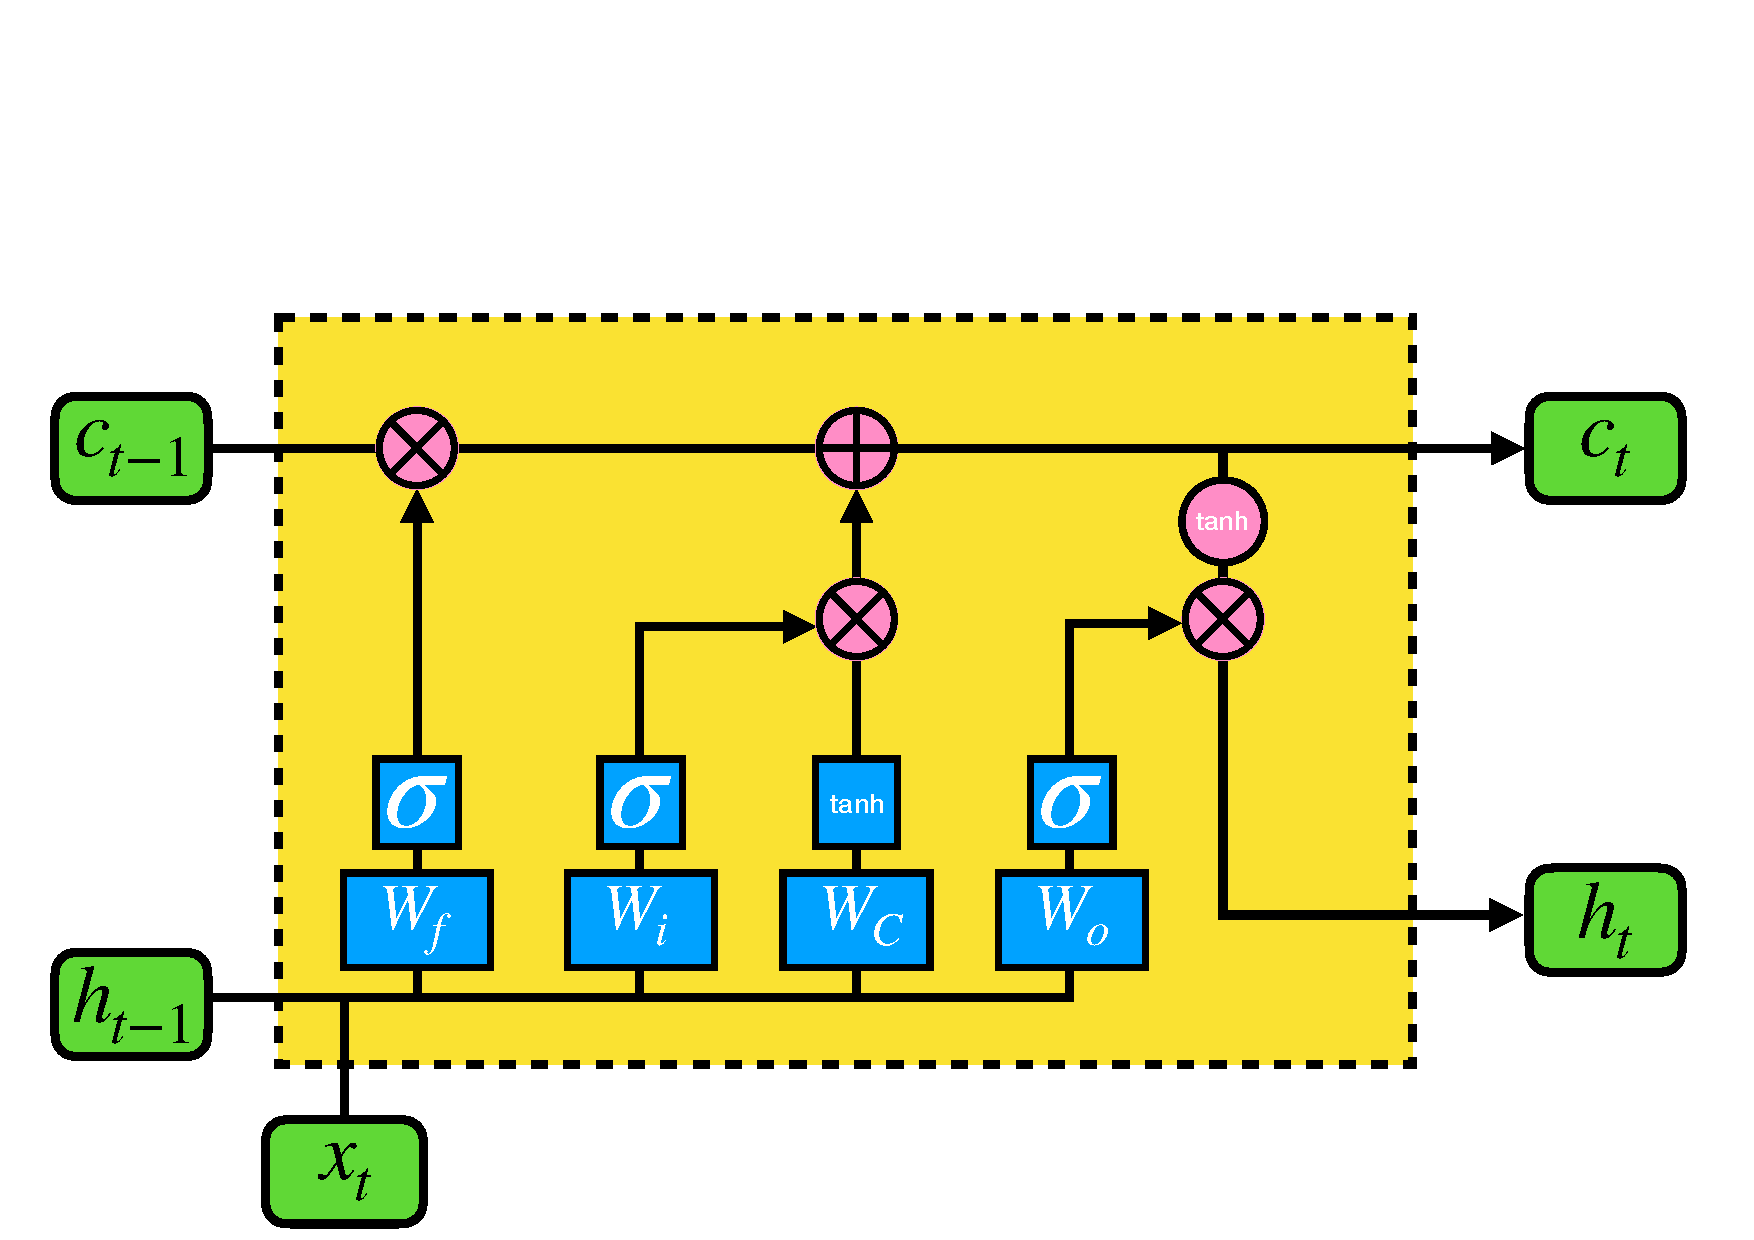
\includegraphics[width=0.7\textwidth]{logos/ClassicalLSTM_Diagram.pdf}
\caption[LSTM cell diagram]{A schematic diagram of the classical long short-term memory (LSTM) cell architecture, showing the three gates (forget, input, output) and the cell state pathway. \cite{chen2020quantumlongshorttermmemory}}
\label{fig:lstm_cell_diagram}
\end{figure}

\paragraph{Common Variants and Extensions.} Beyond the basic cell, common variants add peephole connections (letting gates observe \(\mathbf{c}_{t-1}\)/\(\mathbf{c}_t\)), or initialize the forget gate bias positively to encourage longer retention at the start of training. Intuitively, the partial derivative \(\partial \mathbf{c}_t/\partial \mathbf{c}_{t-1} = \mathbf{f}_t\) explains how the forget gate directly scales gradient flow along the cell state pathway; values of \(\mathbf{f}_t\) near one help preserve information and gradients over time.

\paragraph{Computational Cost and Practical Considerations.} If \(\mathbf{x}_t \in \mathbb{R}^{d_x}\), \(\mathbf{h}_t, \mathbf{c}_t \in \mathbb{R}^{d_h}\), each gate uses an affine map with parameters of size \(d_h\times(d_x+d_h)\) plus bias. Four such maps imply a per-step cost of order \(\mathcal{O}(d_h(d_x+d_h))\) and memory proportional to activations over time. In practice, mini-batch computation dominates wall time; masking or packed sequences prevent padded timesteps from contributing spurious gradients.

\paragraph{Gate Saturation Regimes.} When \(\mathbf{f}_t\) saturates near 1 while \(\mathbf{i}_t \approx 0\), the LSTM behaves as a leaky integrator that retains past information; conversely, \(\mathbf{f}_t\) near 0 forgets rapidly. The output gate \(\mathbf{o}_t\) modulates exposure of the internal memory to downstream layers; throttling \(\mathbf{o}_t\) can stabilize training early on at the cost of slower information throughput.

\paragraph{Advanced Training Techniques.} Normalization inside the cell (e.g., layer normalization on gate pre-activations) can reduce covariate shift across time and ease optimization, sometimes enabling larger learning rates. Coupled input–forget gate (CIFG) variants tie \(\mathbf{f}_t = 1-\mathbf{i}_t\) to reduce parameters and encourage complementary behavior; while parameter-efficient, CIFG may be less expressive on tasks requiring independent retention and write controls. Peepholes let gates read the cell state and can improve precise temporal counting.

\paragraph{A short gradient derivation.} By unrolling the cell-state update, one obtains
\begin{align}
\frac{\partial \mathbf{c}_t}{\partial \mathbf{c}_{t-1}} &= \mathbf{f}_t,\quad\; \frac{\partial \mathbf{c}_{t-1}}{\partial \mathbf{c}_{t-2}} = \mathbf{f}_{t-1},\; \ldots \\
\Rightarrow\; \frac{\partial \mathbf{c}_t}{\partial \mathbf{c}_{t-k}} &= \prod_{j=t-k+1}^{t} \mathbf{f}_j.
\end{align}
When the forget gates are near one, this multiplicative path preserves gradients over long spans; when they are small, information is intentionally forgotten.

\paragraph{LSTM forward steps (per time \(t\)).} Given \(\mathbf{x}_t\) and \((\mathbf{h}_{t-1},\mathbf{c}_{t-1})\): (1) compute gates \(\mathbf{f}_t,\mathbf{i}_t,\mathbf{o}_t\) and candidate \(\tilde{\mathbf{c}}_t\); (2) update memory \(\mathbf{c}_t = \mathbf{f}_t\odot\mathbf{c}_{t-1}+\mathbf{i}_t\odot\tilde{\mathbf{c}}_t\); (3) expose state \(\mathbf{h}_t = \mathbf{o}_t\odot \tanh(\mathbf{c}_t)\). Mini-batch masking ensures padded steps neither affect gate activations nor the loss.

\subsection{LSTM Variants and Training Techniques}
Beyond the vanilla cell, a number of practical variants and training techniques are widely adopted to improve optimization stability and efficiency:
\begin{itemize}
    \item \textbf{Peephole connections} let gates access the cell state \(\mathbf{c}_{t-1}\) or \(\mathbf{c}_t\) directly, tightening control over precise counting and timing \citep{gers2000learning}. This variant has shown improvements in tasks requiring precise temporal modeling.
    \item \textbf{Coupled input–forget gate (CIFG)} ties \(\mathbf{f}_t = 1-\mathbf{i}_t\) to reduce parameters and encourage complementary behavior; while parameter-efficient, decoupled gates can be more expressive when retention and writing need to be controlled independently \citep{greff2017lstm}.
    \item \textbf{Normalization in RNNs} (e.g., layer normalization applied to gate pre-activations) reduces internal covariate shift and can enable larger learning rates and deeper stacks \citep{ba2016layer}. Recent work has shown significant improvements in training stability and convergence speed.
    \item \textbf{Recurrent dropout/Zoneout}. Instead of dropping inputs only, apply structured noise on recurrent connections or randomly preserve previous hidden states to regularize temporal dynamics while keeping information flow stable \citep{krueger2017zoneout, semeniuta2016recurrent}.
    \item \textbf{Initialization and clipping}. Orthogonal initialization of \(\mathbf{W}_{hh}\), positive bias for forget gates, and global-norm gradient clipping (e.g., 0.5--5.0) are common to mitigate exploding gradients \citep{pascanu2013difficulty, jozefowicz2015empirical}.
    \item \textbf{Packing/masking}. For variable-length sequences, use padding masks (or packed sequences) to prevent padded steps from contributing to attention, gates, or the loss \citep{goodfellow2016deep}.
\end{itemize}
Stacking 2--3 LSTM layers with residual or skip connections often improves representation power with modest overhead \citep{he2016deep}. In industrial time-series, stacking is typically combined with temporal pooling or attention to summarize features for classification \citep{zhao2019deep}.

\subsection{Strengths and Limitations for Time-Series Modeling}
\textbf{Strengths.} LSTMs are effective at modeling sequential dependencies, handling variable-length inputs, and integrating multivariate sensor streams. Their gating mechanism helps filter noise and retain salient temporal patterns, which has led to strong results in industrial time-series fault detection and prediction \cite{filonov2016multivariateindustrialtimeseries, zhao2019deep}. They naturally support many-to-one (sequence classification), many-to-many (sequence labeling), and sequence-to-sequence settings. In practice, padding and masking let LSTMs consume mini-batches of variable-length sequences without corrupting gradients. When paired with dropout/Zoneout and early stopping, LSTMs generalize well on moderately sized datasets.

\textbf{Limitations.} Despite improved gradient flow, LSTMs can still struggle with very long sequences and long-range interactions spanning hundreds or thousands of steps. Their inherently sequential computation limits parallelism on modern accelerators, yielding higher training latency and memory usage compared with attention-based models. Performance can be sensitive to depth, hidden size, and regularization choices; small datasets may overfit without proper constraints. Moreover, when global context is crucial, attention-based architectures such as the Transformer can capture long-range dependencies more efficiently via direct pairwise interactions and highly parallel computation \cite{pascanu2013difficulty, vaswani2017attention}. In forecasting, encoder-decoder hybrids (e.g., LSTM encoder with attention) are often adopted to mitigate these limitations.

\textbf{Implementation notes.} Normalization (z-score per channel), careful learning-rate schedules (e.g., cosine decay with warmup), and gradient clipping thresholds tuned between 0.5 and 5.0 are common. For class-imbalanced fault data, weighted losses or focal loss can complement LSTM modeling; early anomaly detection may benefit from shorter truncation windows updated more frequently, whereas long-horizon forecasting uses longer windows at the expense of compute.

\textbf{Data windowing and leakage.} For supervised time-series learning, choose window length and stride to reflect the process dynamics (e.g., at least a few dominant periods of vibration). Ensure no temporal leakage from future segments into training windows for validation/test splits; use contiguous block splits when distribution shift over time is plausible. Missing values can be handled with masking inputs and, optionally, time-since-last-observation channels to inform the model about gaps.

\begin{table}[t]
\centering
\caption{Typical LSTM configuration choices (indicative ranges; tune on validation).}
\label{tab:lstm_config}
\begin{tabular}{l l}
\hline
Hidden size \(d_h\) & 64--256, increase with data size/complexity \\
Layers & 1--3 (stacked), residual skip if \(\geq 3\) \\
Dropout & 0.1--0.5 between layers (avoid inside gates) \\
Truncated BPTT \(K\) & 50--200 steps depending on context length \\
Clip norm & 0.5--5.0 (global \(\ell_2\)) \\
LR & \(10^{-3}\) to \(10^{-4}\) with Adam/decoupled weight decay \\
Batching & Pad + mask or packed sequences to handle variable length \\
\hline
\end{tabular}
\end{table}

\begin{table}[t]
\centering
\caption{Qualitative comparison of sequence models for industrial time-series.}
\label{tab:model_compare}
\begin{tabular}{p{2.8cm} p{3.2cm} p{3.2cm} p{3.8cm}}
\hline
\textbf{Aspect} & \textbf{LSTM} & \textbf{GRU} & \textbf{Transformer} \\
\hline
Parameters & Higher (4 gates) & Lower (3 gates) & High (attention blocks) \\[0.5ex]
Parallelism & Low (sequential) & Low (sequential) & High (token-parallel) \\[0.5ex]
Long-range dependencies & Moderate (via gates) & Moderate & Strong with attention \\[0.5ex]
Latency (causal) & Good (uni-directional) & Good (uni-directional) & Moderate (causal masks) \\[0.5ex]
Data requirements & Moderate & Moderate & Higher for stability \\
\hline
\end{tabular}
\end{table}

\subsection{Bidirectional LSTM (Bi-LSTM)}
Bi-LSTM extends the standard LSTM by running two LSTMs in parallel: one processes the sequence forward (from \(t=1\) to \(T\)) and the other backward (from \(t=T\) to \(1\)). The two hidden representations are then concatenated (or combined) to form a context-enriched feature at each time step. This provides the model with information from both past and future contexts, which often improves performance on sequence classification and labeling tasks where the full sequence is available at inference time. However, Bi-LSTM is not causal and thus unsuitable for strict real-time scenarios that cannot access future observations. In machinery health monitoring and fault diagnosis, Bi-LSTMs have been widely adopted as a strong baseline due to their enhanced context modeling capability \cite{zhang2019deep, zhao2019deep}.

\begin{figure}[!h]
\centering
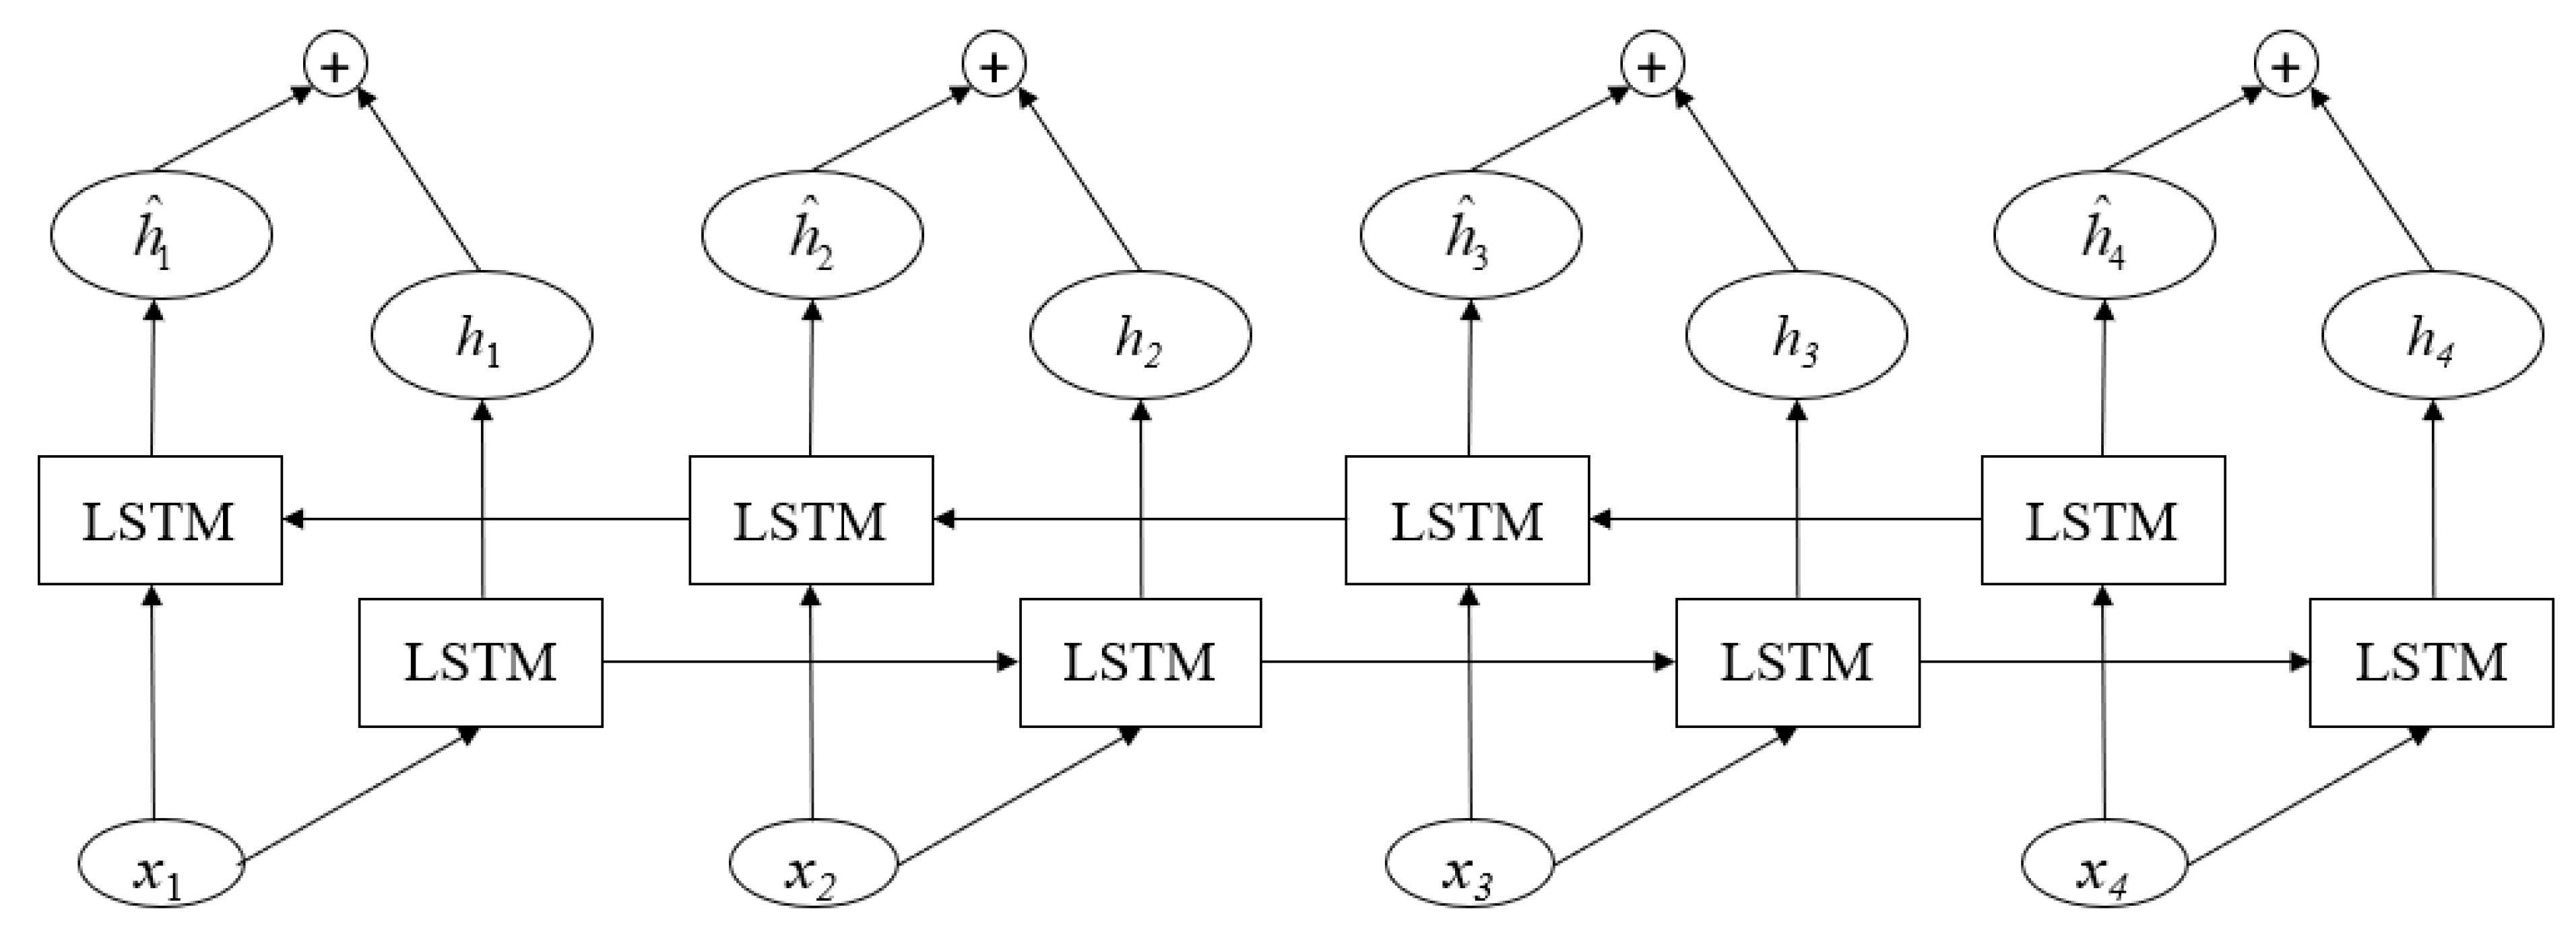
\includegraphics[width=0.8\textwidth]{logos/BI-LSTM.png}
\caption[Bidirectional LSTM architecture]{A schematic diagram of the bidirectional LSTM (Bi-LSTM) architecture\cite{s21206758}}
\end{figure}

In practice, Bi-LSTMs are commonly followed by temporal pooling (e.g., max/mean over time) or attention layers to summarize step-wise representations into a fixed-size vector for downstream classification. The bidirectional setup increases parameters and compute compared to a single-direction LSTM, so batch size and sequence length may need tuning to fit memory constraints. For causal or low-latency systems, a uni-directional LSTM (or streaming variants) is preferred.

Formally, if the forward and backward hidden states at step \(t\) are \(\overrightarrow{\mathbf{h}}_t\) and \(\overleftarrow{\mathbf{h}}_t\), a common fusion is concatenation \(\mathbf{z}_t = [\overrightarrow{\mathbf{h}}_t;\,\overleftarrow{\mathbf{h}}_t]\) followed by a classifier \(\mathbf{y}_t = g(\mathbf{W}\mathbf{z}_t + \mathbf{b})\). Pooling over \(t\) or selecting the last step yields sequence-level predictions. Memory and compute roughly double versus a single-direction LSTM with the same \(d_h\).
\par
Where strict causality is not required but low latency matters, limited look-ahead (e.g., a few timesteps) can approximate bidirectional context in streaming by buffering short chunks. For structured sequence labeling (e.g., event boundary detection), a Bi-LSTM encoder paired with a CRF decoding layer can enforce label consistency over time; in classification, simple temporal pooling often suffices.

Conceptually, a Bi-LSTM processes each input step with a forward and a backward LSTM; their hidden states are concatenated and passed to a classifier or pooling layer.


\section{Transformer Model}
\label{sec:related_technologies:transformer}

The Transformer, introduced by \cite{vaswani2017attention}, represents a paradigm shift in sequence modeling, moving away from recurrent architectures and embracing self-attention as its core mechanism. This allows for significantly more parallelization and has established new standards in natural language processing and beyond \citep{zhou2021informer, zhao2019deep}. This section details the foundational concepts of the Transformer, including the attention mechanism, its multi-head variant, and the overall architecture of the encoder block.

\subsection{The Basic Idea of the Attention Mechanism}
The attention mechanism was developed to address the limitations of fixed-length context vectors in traditional encoder-decoder models, where the decoder had to rely on a single vector summarizing the entire input sequence. Attention provides a solution by allowing the model to dynamically focus on different parts of the input sequence when producing an output at a specific time step.

The core idea is to compute a set of attention weights for each element in the input sequence. These weights determine the importance of each input element relative to the current output position. The final output is then a weighted sum of the input representations, where the weights are the computed attention scores. This mechanism enables the model to selectively draw upon the most relevant information from the input, regardless of its position, thereby improving its ability to handle long-range dependencies.
Classical formulations of attention in encoder–decoder models trace back to \cite{bahdanau2015neural}, while modern scaled dot-product attention popularized by \cite{vaswani2017attention} enables highly parallel computation.

\subsection{The Calculation Process of the Self-Attention Mechanism}
Self-attention, also known as intra-attention, is a specific type of attention mechanism that allows a model to weigh the importance of different words within the same sequence. Instead of relating an input and an output sequence, it relates different positions of a single sequence to compute a representation of that sequence.

The calculation is based on three vectors derived from each input embedding: the Query (\(\mathbf{Q}\)), the Key (\(\mathbf{K}\)), and the Value (\(\mathbf{V}\)). These vectors are generated by multiplying the input embedding by three distinct weight matrices.
The process can be summarized in three steps:
\begin{enumerate}
    \item \textbf{Compute Scores:} The score for each position is calculated by taking the dot product of the Query vector of the current position with the Key vectors of all positions in the sequence. This determines how much attention the current position should pay to every other position.
    \item \textbf{Scale and Normalize:} The scores are scaled down by dividing by the square root of the dimension of the key vectors, \(\sqrt{d_k}\). This scaling prevents the dot products from growing too large and pushing the softmax function into regions with very small gradients. A softmax function is then applied to the scaled scores to obtain the attention weights, which are positive and sum to one.
    \item \textbf{Compute Output:} The final output for the position is a weighted sum of the Value vectors, where the weights are the normalized attention scores from the previous step.
\end{enumerate}
This entire computation is captured compactly in the following equation:
\begin{equation}
    \text{Attention}(\mathbf{Q}, \mathbf{K}, \mathbf{V}) = \text{softmax}\left(\frac{\mathbf{Q}\mathbf{K}^T}{\sqrt{d_k}}\right)\mathbf{V}
    \label{eq:self_attention}
\end{equation}

\subsection{The Advantages of Multi-Head Attention}
A single self-attention mechanism can be limiting, as it only allows the model to focus on other positions in one way. The Transformer enhances this by introducing Multi-Head Attention. Instead of performing a single attention function, this mechanism runs multiple attention calculations in parallel.

The primary advantages of this approach are:
\begin{itemize}
    \item \textbf{Diverse Representations:} Each "head" uses different, learned linear projections to transform the input Queries, Keys, and Values. This allows each head to learn to attend to different types of relationships or information from different representation subspaces. For example, one head might learn to capture syntactic relationships, while another focuses on semantic ones.
    \item \textbf{Enriched Feature Combination:} The outputs of all the parallel attention heads are concatenated and passed through a final linear projection. This allows the model to combine the various learned relationships into a single, richer representation for each position.
\end{itemize}

\begin{figure}[htb]
\centering
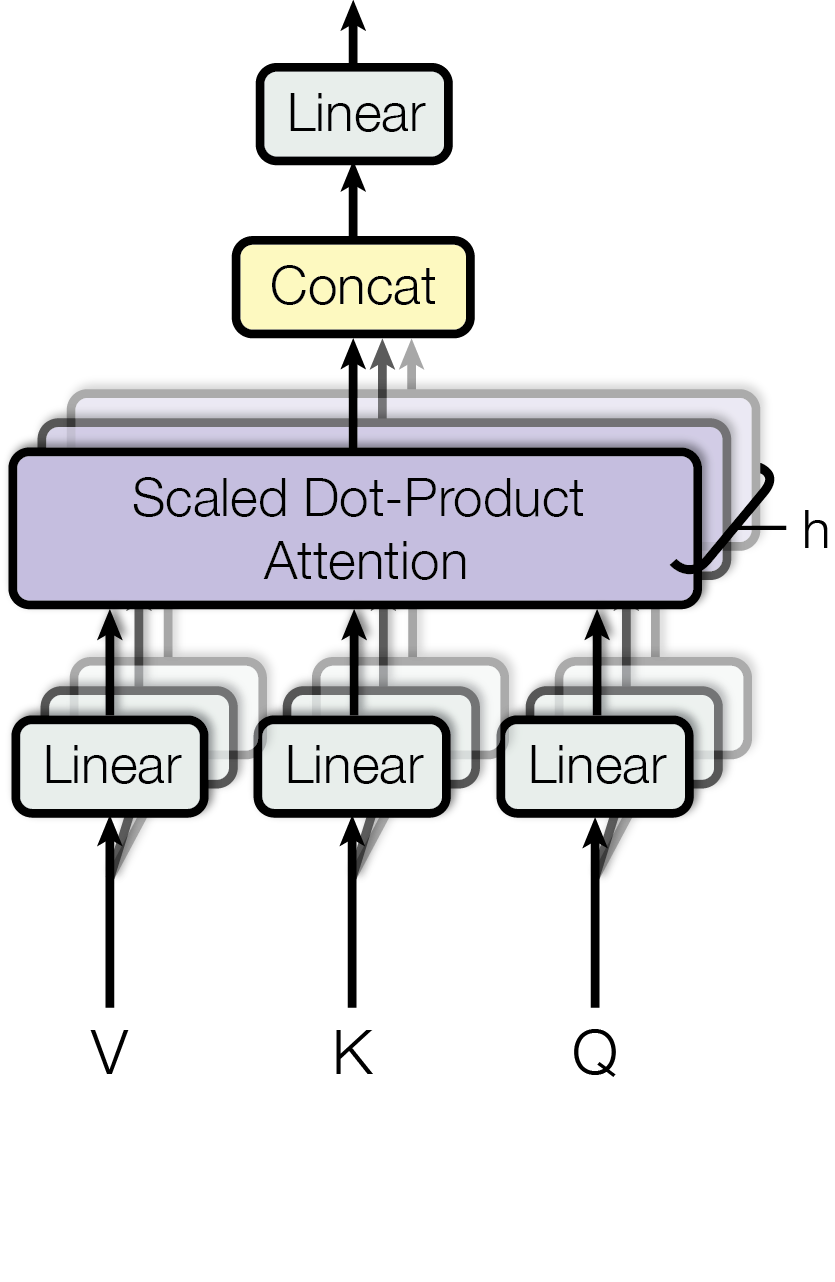
\includegraphics[width=0.3\textwidth]{logos/Multi-head.png}
\caption[Multi-Head Attention mechanism]{Multi-Head Attention consists of several attention layers running in parallel.\cite{vaswani2017attention}}
\label{fig:multi_head_attention}
\end{figure}

In essence, Multi-Head Attention gives the model a broader and more nuanced understanding of the sequence by allowing it to jointly attend to information from different perspectives simultaneously \cite{vaswani2017attention}.

\subsection{The Structure of the Transformer's Encoder}
The Transformer encoder is a stack of identical layers. Each layer is composed of two main sub-layers: a Multi-Head Self-Attention mechanism and a simple, position-wise fully connected Feed-Forward Network (FFN).

Key components of the encoder architecture include:
\begin{itemize}
    \item \textbf{Positional Encoding:} Since the Transformer contains no recurrence or convolution, it has no inherent sense of sequence order. To address this, positional encodings are added to the input embeddings at the bottom of the encoder stack. These are vectors that provide information about the relative or absolute position of tokens in the sequence. The original paper used sine and cosine functions of different frequencies for this purpose \citep{vaswani2017attention}.
    \item \textbf{Feed-Forward Network (FFN):} This sub-layer consists of two linear transformations with a ReLU activation in between: \(\text{FFN}(x) = \max(0, xW_1 + b_1)W_2 + b_2\). It is applied to each position separately and identically, allowing the model to introduce non-linearity and further process the representations from the attention layer \citep{vaswani2017attention}.
    \item \textbf{Residual Connections and Layer Normalization:} Each of the two sub-layers (Multi-Head Attention and FFN) in an encoder layer has a residual connection around it, followed by a layer normalization step. The output of each sub-layer is thus \(\text{LayerNorm}(x + \text{Sublayer}(x))\), where \(\text{Sublayer}(x)\) is the function implemented by the sub-layer itself. These two components are critical for enabling the training of deep Transformer models by stabilizing the learning process and ensuring proper gradient flow \citep{ba2016layer}.
\end{itemize}

\begin{figure}[tb]
\centering
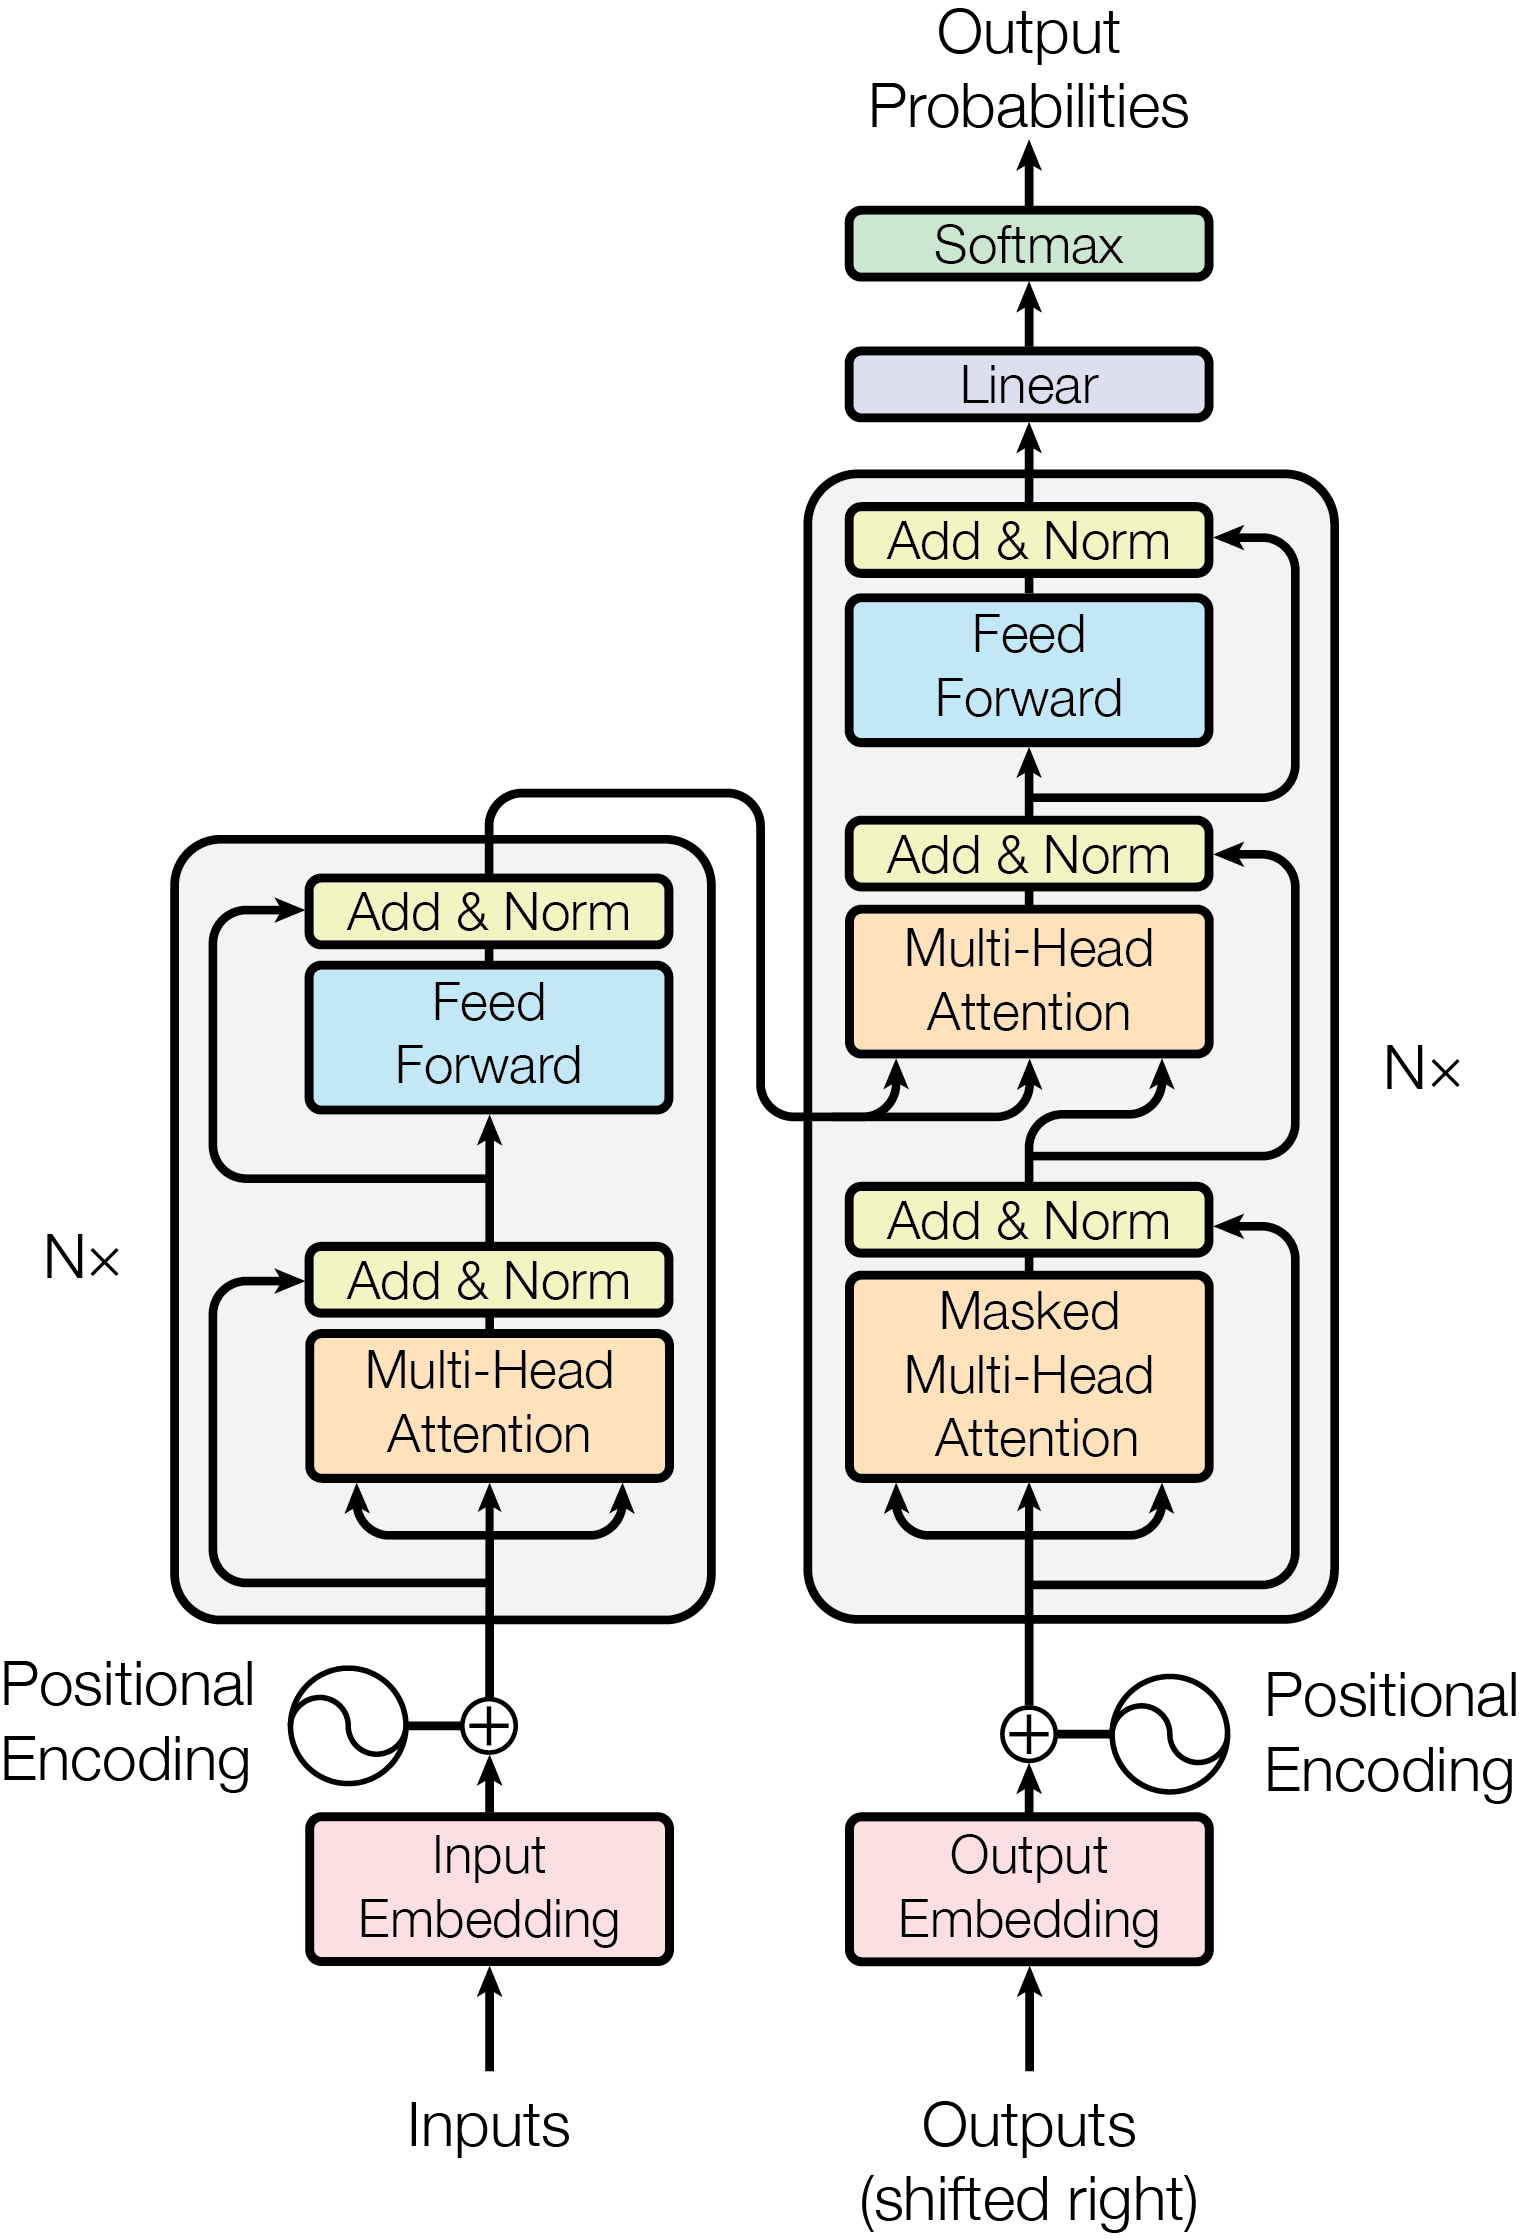
\includegraphics[width=0.5\textwidth]{logos/transformer.png}
\caption[Transformer encoder architecture]{The structure of the Transformer encoder, showing the multi-head self-attention mechanism, feed-forward network, residual connections, and layer normalization components \cite{vaswani2017attention}.}
\label{fig:transformer_encoder}
\end{figure}

As illustrated in Figure~\ref{fig:transformer_encoder}, the Transformer encoder processes input sequences through a stack of identical layers, each containing two main components: a multi-head self-attention mechanism that enables the model to attend to different positions within the sequence, and a position-wise feed-forward network that applies non-linear transformations. The residual connections around each sub-layer, combined with layer normalization, facilitate stable training and effective gradient flow through the deep architecture. This design allows for highly parallelizable computation while capturing complex dependencies across the entire input sequence.



Table~\ref{tab:efficient_attention} summarizes several prominent approaches to reducing the computational complexity of self-attention mechanisms. While standard Transformer attention requires $\mathcal{O}(T^2 d)$ operations for sequence length $T$ and model dimension $d$, these variants achieve sub-quadratic complexity through different approximation strategies. Linformer reduces complexity by projecting the sequence dimension to a lower rank $r$, Performer employs kernel feature maps to linearize attention computation, and Informer uses sparse attention patterns optimized for long-sequence forecasting tasks. These efficiency improvements are particularly relevant for processing long time-series sequences in industrial applications.

\subsection{Positional Encodings and Masking Variants}
While fixed sinusoidal encodings are widely used, alternative schemes exist: \emph{learned} absolute positional embeddings, and \emph{relative} position representations that parameterize pairwise bias as a function of offset, often improving generalization to longer sequences and enabling translation invariance in attention \citep{shaw2018self}. For time-series, seasonal patterns can be injected via multi-scale encodings (e.g., combining periodic sinusoids at different frequencies), and \emph{time-delta} channels can inform the model about irregular sampling.\par
Masking controls information flow. \textbf{Padding masks} prevent attending to padded tokens; \textbf{causal masks} enforce uni-directionality for forecasting/streaming; \textbf{block/local masks} constrain receptive fields to reduce computation while retaining inductive bias for locality.

\subsection{Complexity and Efficient Transformer Variants}
Full self-attention scales as \(\mathcal{O}(T^2 d)\) in time and \(\mathcal{O}(T^2)\) in memory for sequence length \(T\) and model width \(d\), which can be prohibitive for long signals. A line of work proposes sub-quadratic approximations: \textbf{Linformer} projects Keys/Values to a lower rank along the sequence dimension achieving linear complexity in \(T\) \citep{wang2020linformer}; \textbf{Performer} uses randomized feature maps to approximate softmax attention with linear-time kernel attention \citep{choromanski2021rethinking}; \textbf{Informer} exploits ProbSparse attention and top-$k$ queries to reduce cost in long-horizon forecasting \citep{zhou2021informer}. These designs trade a small approximation error for significant speed/memory savings.

\begin{table}[h]
\centering
\caption{Selected efficient attention variants (conceptual summary).}
\label{tab:efficient_attention}
\begin{tabular}{l l l}
\hline
Method & Core idea & Complexity vs. full \\ \hline
Linformer & Low-rank proj. on sequence axis & \(\mathcal{O}(T d r)\) \\
Performer & Kernel feature maps for attention & \(\mathcal{O}(T d^2)\) \\
Informer & ProbSparse/top-$k$ queries & \(\mathcal{O}(T \log T)\) (approx.) \\ \hline
\end{tabular}
\end{table}

\subsection{Architectural Variants for Different Tasks}
\textbf{Encoder-only} stacks (e.g., BERT-style) suit representation learning and classification; \textbf{decoder-only} stacks with causal masks suit autoregressive modeling and forecasting; \textbf{encoder--decoder} designs enable sequence-to-sequence mapping and cross-attention fusion from context to targets. In industrial fault diagnosis, encoder-only Transformers with a classification head are common; for forecasting, causal decoder-only or encoder--decoder architectures are preferred, with appropriate masking.


% --- BEGINNING OF LATEX SECTION ---

% 建议在您的LaTeX文档序言部分确保包含以下包:
% \usepackage{amsmath} % 用于数学环境
% \usepackage{natbib}  % 用于 \citep 等引文命令

\section{Key Technologies in Deep Learning}
\label{sec:key_technologies}

The success of a deep learning model is not solely dependent on its architecture but is profoundly influenced by the synergistic application of several key technologies during the training process. These technologies guide the model's learning, enhance its efficiency, and ensure its ability to generalize to new, unseen data. This section elaborates on the critical components adopted in this research: the loss function chosen to handle data imbalances, the optimization algorithm that drives model convergence, and the regularization techniques employed to combat overfitting.

\subsection{Loss Function: From Cross-Entropy to Focal Loss}
\label{sec:loss_functions}

The loss function serves as the objective for optimization, quantifying the discrepancy between the model's predictions and the ground truth. A well-chosen loss function is paramount for directing the model's learning toward the desired outcome.

\textbf{Cross-Entropy (CE) Loss} is the de facto standard for multi-class classification tasks. It originates from information theory and measures the dissimilarity between two probability distributions: the predicted probability distribution from the model and the true distribution (represented as a one-hot vector). For a single sample, the CE loss is formulated as:
\begin{equation}
\text{CE}(p, y) = - \sum_{i=1}^{C} y_i \log(p_i)
\label{eq:ce_loss}
\end{equation}
where $C$ is the number of classes, $y_i$ is 1 if the sample belongs to class $i$ and 0 otherwise, and $p_i$ is the model's predicted probability for class $i$. While effective in balanced scenarios, CE loss exhibits a significant drawback when faced with \textbf{class imbalance}. In many real-world datasets, such as those in machinery fault diagnosis, normal-condition samples vastly outnumber faulty-condition samples. In such cases, the total loss becomes dominated by the easily classified, high-frequency majority class, leading to a model that is biased and performs poorly on the very classes of interest.

To counteract this, this study employs \textbf{Focal Loss (FL)}, an elegant modification of the standard Cross-Entropy loss \citep{lin2017focal}. Focal Loss dynamically reshapes the loss function to concentrate the training effort on ``hard'' or misclassified examples. It achieves this by introducing a modulating factor to the CE loss:
\begin{equation}
\text{FL}(p_t) = - \alpha_t (1 - p_t)^\gamma \log(p_t)
\label{eq:focal_loss}
\end{equation}
Here, $p_t$ represents the model's estimated probability for the ground-truth class. The key components are:
\begin{enumerate}
    \item \textbf{The Modulating Factor $(1 - p_t)^\gamma$}: This is the core innovation. When a sample is easily classified ($p_t \to 1$), the term $(1 - p_t)$ approaches 0. Raising this to a power $\gamma > 0$ (e.g., $\gamma = 2$) causes the loss contribution of this easy sample to be drastically reduced. Conversely, for a hard sample ($p_t \to 0$), the modulating factor approaches 1, and its loss is preserved. The \textbf{focusing parameter $\gamma$} smoothly adjusts the rate at which easy examples are down-weighted.
    \item \textbf{The Balancing Factor $\alpha_t$}: This is a weighting factor that directly addresses class frequency by assigning a higher weight to minority classes. It provides a static baseline for balancing, which is then dynamically refined by the modulating factor.
\end{enumerate}
By adopting Focal Loss, we equip our model to effectively learn from imbalanced data, ensuring that the rare but crucial fault signatures are not ignored during training.

\subsection{Optimization Algorithm: Adam}
\label{sec:optimizer_adam}

The optimization algorithm is the engine that updates the model's parameters to minimize the loss function. This research utilizes the \textbf{Adam (Adaptive Moment Estimation)} optimizer, a highly effective and widely used algorithm \citep{kingma2014adam}. Adam combines the strengths of two other popular methods: Momentum and RMSprop. It maintains an exponentially decaying average of past gradients (first moment) and past squared gradients (second moment). This allows it to compute individual, adaptive learning rates for different parameters, leading to faster convergence and robust performance across a wide range of deep learning models.

\paragraph{Learning-rate schedules and decoupled weight decay.} Beyond vanilla Adam, \textbf{AdamW} decouples weight decay from the gradient-based update, often yielding better regularization than L2 penalties baked into the loss \citep{loshchilov2019decoupled}. Practical schedules include \textbf{cosine annealing with warm restarts} to escape sharp minima \citep{loshchilov2016sgdr} and the \textbf{OneCycle} policy to traverse a wider range of learning rates/momenta for faster convergence \citep{smith2018superconvergence}. Warmup (a brief linear increase of learning rate at the start) is especially helpful for attention models.

\subsection{Regularization Techniques: Dropout and Weight Decay}
\label{sec:regularization}

A primary challenge in training deep networks is \textbf{overfitting}. To mitigate this risk, we employ two powerful regularization techniques.

\textbf{Dropout} is a method that prevents complex co-adaptations on training data \citep{srivastava2014dropout}. During each training iteration, it randomly sets the outputs of a fraction of neurons to zero. This forces the network to learn more robust features and acts as a form of model averaging.

\paragraph{Data augmentation for time series.} Augmentations such as jittering (Gaussian noise), scaling, magnitude warping, time warping, permutation, and window slicing can improve robustness and reduce overfitting; MixUp/CutMix analogues on temporal signals must be applied with care to preserve label semantics. A recent survey systematizes augmentation choices for time-series deep learning \citep{wen2021time}.

\paragraph{Handling class imbalance beyond Focal Loss.} In addition to Focal Loss, re-sampling (minority oversampling/majority undersampling), synthetic sample generation (e.g., SMOTE \citep{chawla2002smote}), or class-balanced re-weighting by effective number of samples are commonly used. Threshold moving and calibrating decision thresholds on a validation set can further improve minority-class recall without inflating false positives excessively.

\paragraph{Evaluation metrics and reporting.} For multi-class fault diagnosis under imbalance, accuracy alone can be misleading. We report macro-averaged Precision/Recall/F1 and ROC/PR curves. For a class \(c\),
\begin{align}
\mathrm{Precision}_c &= \frac{\mathrm{TP}_c}{\mathrm{TP}_c + \mathrm{FP}_c},\quad
\mathrm{Recall}_c = \frac{\mathrm{TP}_c}{\mathrm{TP}_c + \mathrm{FN}_c},\\
\mathrm{F1}_c &= \frac{2\,\mathrm{Precision}_c\,\mathrm{Recall}_c}{\mathrm{Precision}_c+\mathrm{Recall}_c}.
\end{align}
Macro-averaging treats all classes equally by averaging the per-class scores; micro-averaging aggregates TP/FP/FN across classes before computing the metrics, favoring frequent classes. Confusion matrices complement these metrics by revealing dominant error modes.

\textbf{Weight Decay}, most commonly implemented as \textbf{L2 Regularization}, adds a penalty term to the loss function proportional to the squared magnitude of the model's weights:
\begin{equation}
L_{\text{new}} = L_{\text{original}} + \frac{\lambda}{2} \sum_{w} w^2
\label{eq:l2_reg}
\end{equation}
This penalty encourages the model to find solutions with smaller weights, which typically leads to a less complex model with better generalization performance \citep{goodfellow2016deep}.


\section{Chapter Summary}
\label{sec:related_technologies:summary}

This chapter introduced core sequence models with a focus on LSTMs. We explained why plain RNNs suffer from vanishing/exploding gradients and how the LSTM’s additive cell state with multiplicative gates alleviates this, enabling learning of longer dependencies. The remaining Figure~\ref{fig:lstm_cell_diagram} illustrated the LSTM cell and its forget/input/output gates, serving as a visual complement to the gating equations. We also discussed LSTM strengths and limitations for time-series tasks and the role of Bi-LSTMs when non-causal, bidirectional context is available.
